We recall that our goal is to compute the expectation in \eqref{BS_formula_rbergomi}. In fact, as seen in Section \ref{sec:Simulation of the rBergomi model}, we need   $2N$ dimensional Gaussian inputs for the used  hybrid  scheme ($N$ is the number of time steps in  the time grid), namely
\begin{itemize}
	\item $\mathbf{W}^{(1)}=\{W^{(1)}_i\}_{i=1}^N$: The $N$ Gaussian random variables that are defined in Section  \ref{sec:The rBergomi model}.
	\item $\mathbf{W}^{(2)}=\{W^{(2)}_j\}_{j=1}^N$: An artificial introduced $N$ Gaussian random variables that are used for left-rule points in the hybrid scheme, as explained in Section  \ref{sec:Simulation of the rBergomi model}.
\end{itemize}

Thus, we can rewrite \eqref{BS_formula_rbergomi} as 


\begin{align}\label{BS_formula_rbergomi_2}
C_{\text{RB}}\left( T, K \right)&=\text{E}\left[C_{\text{BS}}\left( S_0 = \operatorname{exp}\left(\rho \int_0^T \sqrt{v_t} dW_t^1 - \frac{1}{2}
\rho^2 \int_0^T v_t dt\right),\ k = K, \ \sigma^2 = (1-\rho^2)
\int_0^T v_t dt \right) \right], \nonumber \\
&\approx \int_{\rset^{2N}} C_{BS} \left(G(\mathbf{W}^{(1)},\mathbf{W}^{(2)})\right) \rho_{N}(\mathbf{W}^{(1)})  \rho_{N}(\mathbf{W}^{(2)}) d\mathbf{W}^{(1)} d\mathbf{W}^{(2)}:=C_{RB}^{N},
\end{align}

where $G$  maps  $2N$ independent standard Gaussian random inputs to the parameters fed to Black-Scholes formula as in \eqref{BS_formula_rbergomi_2}, and  $\rho_N$ is the multivariate Gaussian density, given by 

\begin{equation*}\label{eq: multivariate gaussian distribution}
\rho_N(\mathbf{z})=\frac{1}{(2 \pi)^{N/2}} e^{-\frac{1}{2} \mathbf{z}^T \mathbf{z}} \PERIOD
\end{equation*} 

Therefore, the initial integration problem that we are solving lives in $2 N$-dimensional space, which becomes very large as the number of time steps $N$, used in the hybrid scheme, increases.


Our approach of approximating the expectation in \eqref{BS_formula_rbergomi_2} is based on multi-index stochastic collocation (MISC), proposed in \cite{haji2016multi}. We describe the  MISC solver in our context in Section \ref{sec:Details of the MISC}.  To make an effective use of MISC, we  first apply two transformations to overcome the issue of facing a high dimensional integrand due to the discretization scheme used for simulating the rBergomi dynamics. The first transformation consists of applying a hierarchical  path generation method, based on Brownian
bridge (Bb) construction, with the aim of reducing the effective dimension as  described  in Section \ref{sec:Brwonian bridge construction}. The second transformation consists of applying Richardson extrapolation to reduce the bias, resulting in reducing  the maximum number of dimensions needed for the integration problem. Details about  Richardson extrapolation  are provided in Section \ref{sec:Richardson extrapolation}.




If we denote by $\mathcal{E}_{\text{tot}}$ the total error of approximating the  expectation in \eqref{BS_formula_rbergomi} using the MISC estimator, $Q_N$, then we have a natural error decomposition, giving by
 
\begin{align}\label{eq:total_error}
\mathcal{E}_{\text{tot}} & \le \abs{C_{\text{RB}}-C_{\text{RB}}^N}+\abs{C_{\text{RB}}^N-Q_{N}}\nonumber\\
  & \le \mathcal{E}_B(N)+ \mathcal{E}_Q(\text{TOL}_{\text{MISC}},N),
\end{align}
where  $\mathcal{E}_Q$ is the quadrature error, a function of the MISC tolerance:  $\text{TOL}_{\text{MISC}}$ and $N$: the number of time steps, $\mathcal{E}_B$  is the bias, function of $N$, and $C_{\text{RB}}^N$ is the biased price computed with $N$ time steps as given by \eqref{BS_formula_rbergomi_2}.

\subsection{The MISC solver}\label{sec:Details of the MISC}

We assume that we want to approximate the expected value $\text{E}[f(Y)]$ of an analytic function $f\colon \Gamma \to \rset$ using a tensorization of quadrature formula over $\Gamma$.

To introduce simplified notations, we start with the one-dimensional case. Let us denote by $\beta \geq 1$ an integer referred to as a ``stochastic discretization level", and by $m: \nset \rightarrow \nset$  a strictly increasing function with $m(0)=0$ and $m(1)=1$, that we call  ``level-to-nodes function". At level $\beta$, we consider a set of $m(\beta)$ distinct quadrature points in $\rset$, $\mathcal{H}^{m(\beta)}=\{y^1_\beta,y^2_\beta,\dots,y_\beta^{m(\beta)}\} \subset \rset$, and a set of quadrature weights, $\boldsymbol{\omega}^{m(\beta)}=\{\omega^1_\beta,\omega^2_\beta,\dots,\omega_\beta^{m(\beta)}\}$. We also let $C^0(\rset)$ be the set of real-valued continuous functions over $\rset$. We then define the quadrature operator as


\begin{equation}
Q(m(\beta)):C^0(\rset) \rightarrow \rset, \quad Q(m(\beta))[f]= \sum_{j=1}^{m(\beta)} f(y^j_\beta) \omega_\beta^j.
\end{equation}





In our case, and following \eqref{BS_formula_rbergomi_2}, we have a multi-variate integration problem and  we have, given the previous notations,    $f:=C_{\text{BS}}\circ G$, $\mathbf{Y}=(\mathbf{W}^{(1)},\mathbf{W}^{(2)})$, and  $\Gamma=\rset^{2N}$.  Therefore,  we define for any multi-index $\boldsymbol{\beta} \in \nset^{2N}$

$$Q^{m(\boldsymbol{\beta})}: \Gamma \rightarrow \rset,\quad  Q^{m(\boldsymbol{\beta})}= \bigotimes_{n = 1}^{2N} Q^{m(\beta_n)} $$

where the $n$-th quadrature operator is understood to act only on the $n$-th variable of $f$. Practically, we obtain the value of $Q^{m(\boldsymbol{\beta})}[f]$  by considering the tensor grid $\mathcal{T}^{m(\boldsymbol{\beta})}= \prod_{n = 1}^{2N}  \mathcal{H}^{m(\beta_n)}$ with cardinality $\#\mathcal{T}^{m(\boldsymbol{\beta})}=\prod_{n=1}^{2N} m (\beta_n)$ and computing

$$ Q^{\mathcal{T}^{m(\boldsymbol{\beta})}}[f]= \sum_{j=1}^{\#\mathcal{T}^{m(\boldsymbol{\beta})}} f(\hat{y}_j) \bar{\omega}_j$$
where $\hat{y}_j \in \mathcal{T}^{m(\boldsymbol{\beta})}$ and $\bar{\omega}_j$ are  products of weights of the univariate quadrature rules.
\begin{remark}
We note that the quadrature points are chosen to optimize the convergence properties of the quadrature error.  For instance, in our context, since we are dealing with Gaussian densities, using Gauss-Hermite quadrature points is the appropriate choice.
\end{remark}

A direct approximation $\expt{f[\mathbf{Y}]} \approx Q^{m(\boldsymbol{\beta})}[f]$ is not an appropriate option  due to the well-known ``curse of dimensionality" effect. We use MISC as in \cite{haji2016multi}, which is a hierarchical adaptive sparse grids quadrature strategy that uses  stochastic discretizations  and classic sparsification approach to obtain an effective approximation scheme for $\expt{f}$. 

 For the sake
of concreteness, in our setting, we are left with a $2N$-dimensional Gaussian random inputs, which are chosen independently, resulting in  $2N$ numerical parameters for MISC, which we use as the basis of the multi-index construction. For a multi-index $\boldsymbol{\beta} = (\beta_n)_{n=1}^{2N} \in \mathbb{N}^{2N}$, we denote  by
$Q_N^{\boldsymbol{\beta}}$,   the result of approximating \eqref{BS_formula_rbergomi_2} with a number of quadrature points  in the $i$-th dimension equal to  $m(\beta_i)$. We further define the set of
differences $\Delta Q_N^{\boldsymbol{\beta}}$ as follows: for a single index $1 \le i \le 2N$,
let

%, reflecting the fact that $W^1_i$ and $W^2_j$ can vary independently of each other regardless of $i \neq j$ or $i = j$. 
%
%Let $ \in \{1, \ldots, 2N\}$ and set
%\begin{equation}
%p_l \coloneqq
%\begin{cases}
%W^1_l, & 1 \le l \le N,\\
%W^2_{l-N}, & N+1 \le l \le 2N.
%\end{cases}
%\end{equation}


%by $\mathbf{m}(\ell)=(m(l_1),\dots, m(l_{2N}))$ the number of quadrature points used in each direction, and  we denote


\begin{equation}
\Delta_i Q_N^{\boldsymbol{\beta}} \coloneqq \left\{ 
\aligned 
 Q_N^{\boldsymbol{\beta}} &- Q_N^{\boldsymbol{\beta}'}  \text{ with } \boldsymbol{\beta}' =\boldsymbol{\beta} - e_i, \text{ if } \boldsymbol{\beta}_i>0 \\
 Q_N^{\boldsymbol{\beta}} &, \quad  \text{ otherwise}
\endaligned
\right.
\end{equation}
where $e_i$ denotes the $i$th $2N$-dimensional unit vector. Then, $\Delta
Q_N^{\boldsymbol{\beta}}$ is defined as
\begin{equation}
\Delta Q_N^{\boldsymbol{\beta}} \coloneqq \left( \prod_{i=1}^{2N} \Delta_i \right) Q_N^{\boldsymbol{\beta}}.
\end{equation}
For instance, when $N = 1$, then 
\begin{multline*}
	\Delta Q_1^{\boldsymbol{\beta}} = \Delta_2 \Delta_1 Q_1^{(\beta_1, \beta_2)} = \Delta_2\left( Q_1^{(\beta_1,
		\beta_2)} - Q_1^{(\beta_1-1,\beta_2)} \right) = \Delta_2 Q_1^{(\beta_1,
		\beta_2)} - \Delta_2 Q_1^{(\beta_1-1,\beta_2)} 
	\\= Q_1^{(\beta_1, \beta_2)} - Q_1^{(\beta_1, \beta_2-1)} - Q_1^{(\beta_1-1, \beta_2)} + Q_1^{(\beta_1-1, \beta_2-1)}.
\end{multline*}

We have the telescoping property
\begin{equation}
C_{RB}^{N}=Q_N^\infty = \sum_{\beta_1=0}^\infty \cdots \sum_{\beta_{2N} = 0}^\infty \Delta
Q_N^{(\beta_1, \ldots, \beta_{2N})} = \sum_{\boldsymbol{\beta} \in \mathbb{N}^{2N}} \Delta Q_N^{\boldsymbol{\beta}}.
\end{equation}


 The MISC estimator used for approximating \eqref{BS_formula_rbergomi_2}, and using a set of multi-indices $\mathcal{I}\subset \nset^{2N}$ is given by
\begin{equation*}
	Q_N^{\mathcal{I}} \coloneqq \sum_{\boldsymbol{\beta} \in \mathcal{I}} \Delta Q_N^{\boldsymbol{\beta}}.
\end{equation*}

The quadrature error in this  case  is given by
\begin{equation}\label{eq:quadrature error}
	\mathcal{E}_Q(\text{TOL}_{\text{MISC}},N) =\abs{Q_N^\infty - Q_N^\mathcal{I}} \le \sum_{\boldsymbol{\beta} \in \mathbb{N}^{2N} \setminus
		\mathcal{I}} \abs{\Delta Q_N^{\boldsymbol{\beta}}}.
\end{equation}

If we denote the computational work at level $\boldsymbol{\beta} = (\beta_1, \ldots, \beta_{2N})$ for adding an increment $\Delta Q_N^{\boldsymbol{\beta}}$
in the telescoping sum by  $\mathcal{W_N^{\boldsymbol{\beta}}}$, then the  construction of the optimal  $\mathcal{I}$ will be done by profit thresholding, i.e.,
for a certain threshold value $\bar{T}$, we add a multi-index $\boldsymbol{\beta}$ to
$\mathcal{I}$ provided that
\begin{equation*}
	\log\left( \frac{\abs{\Delta Q_N^{\boldsymbol{\beta}}}}{\mathcal{W}_N^{\boldsymbol{\beta}}} \right) \le \bar{T}.
\end{equation*}



\begin{remark}
	The choice of the hierarchy of quadrature points, $m(\boldsymbol{\beta})$, is flexible in the MISC solver and can be fixed by the user, depending on the convergence properties of the problem at hand. For instance, for the sake of reproducibility, in our numerical experiments we used a linear hierarchy: $m(\beta)=4 (\beta-1)+1,\: 1 \le \beta $, for results of parameter set $1$ in table \ref{table:Reference solution, using MC with $500$ time steps, of Call option price under rBergomi model, for different parameter constellation.}. For the remaining parameter sets in table  \ref{table:Reference solution, using MC with $500$ time steps, of Call option price under rBergomi model, for different parameter constellation.}, we used a geometric hierarchy: $m(\beta)=2^{\beta-1}+1, \:1 \le \beta $.
\end{remark} 


\begin{remark}
As emphasized in \cite{haji2016multi}, one important requirement to get the optimal performance of MISC solver is to check  the convergence of first and mixed differences operators (See \cite{haji2016multi} for details). We checked this requirement in all our numerical experiments, and for illustration, we show in figures (\ref{fig:first_diff_comp_K_1_H_002}, \ref{fig:second_diff_comp_K_1_H_002}), the convergence of first and second order differences for the case of parameter set $2$ in table \ref{table:Reference solution, using MC with $500$ time steps, of Call option price under rBergomi model, for different parameter constellation.}. 
\end{remark} 

\begin{figure}[h!]
	\centering
	\begin{subfigure}{.4\textwidth}
		\centering
		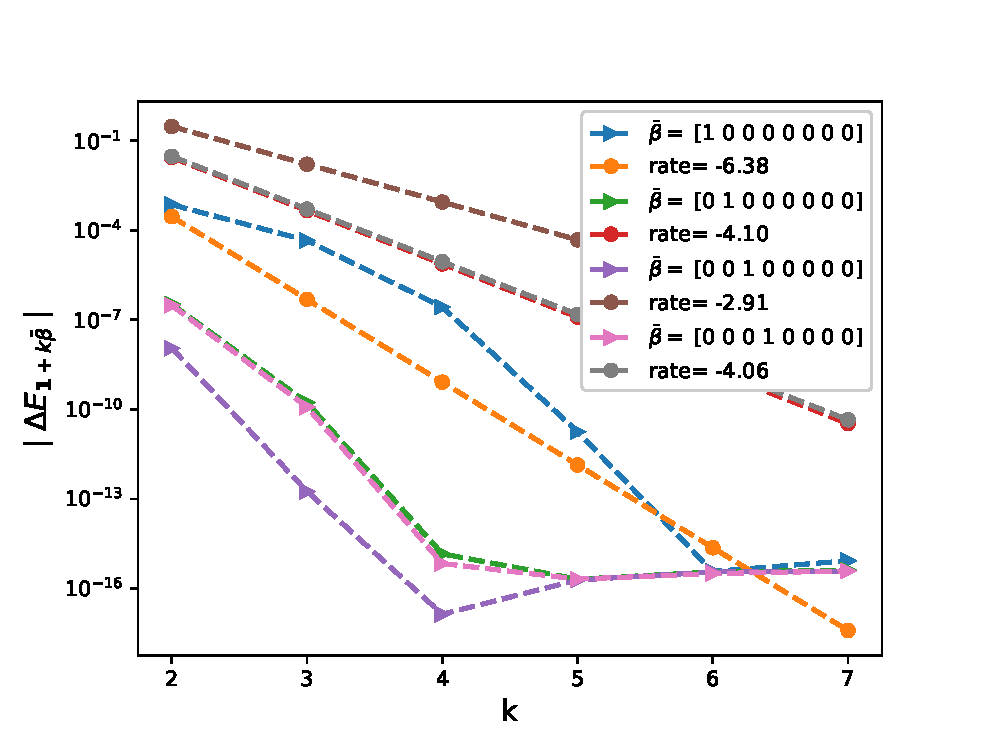
\includegraphics[width=1\linewidth]{./figures/rBergomi_mixed_error_rates/without_change_measure/N_4/H_002/first_difference_rbergomi_4steps_H_002_K_1_totally_hierarch_with_rate_W1}
		\caption{}
		\label{fig:sub3}
	\end{subfigure}%
	\begin{subfigure}{.4\textwidth}
		\centering
		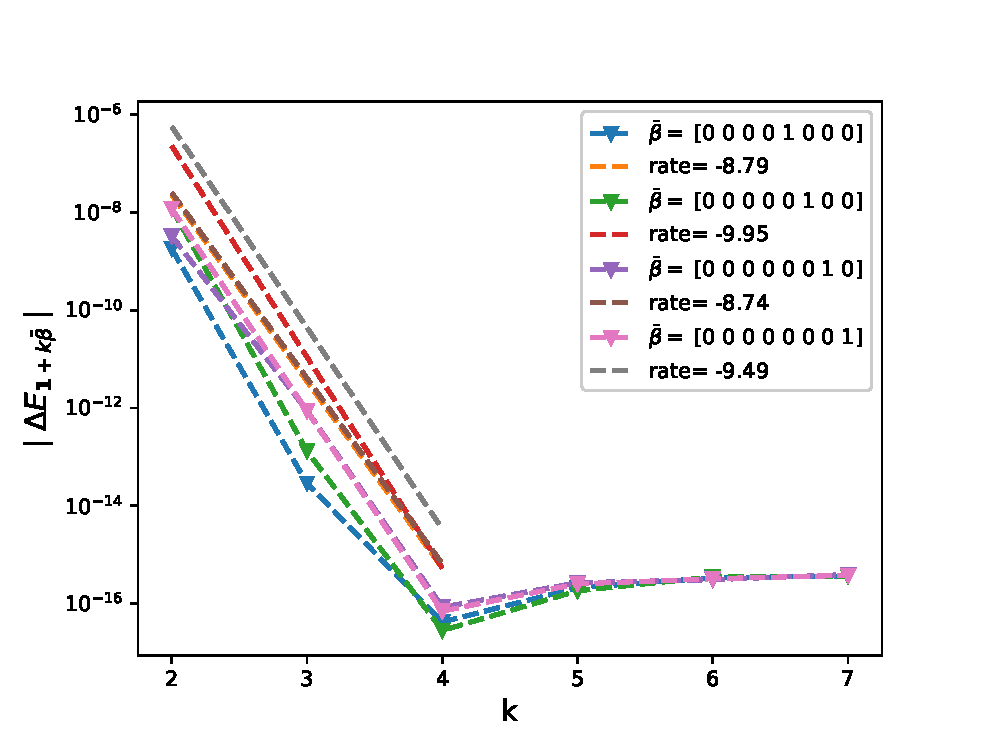
\includegraphics[width=1\linewidth]{./figures/rBergomi_mixed_error_rates/without_change_measure/N_4/H_002/first_difference_rbergomi_4steps_H_002_K_1_totally_hierarch_with_rate_W2}
		\caption{}
		\label{fig:sub4}
	\end{subfigure}
	
	
	
	\caption{The rate of convergence of  first order differences $\abs{\Delta \text{E}_{\beta}}$ ($\beta=\mathbf{1}+k \bar{\beta}$) with respect to $W^{(1)}$ (a)  and  with respect to $W^{(2)}$ (b), for parameter set $2$ in table \ref{table:Reference solution, using MC with $500$ time steps, of Call option price under rBergomi model, for different parameter constellation.}. The number of quadrature points used in the $i$-th dimension is $N_i=2^{\beta_i-1}+1$. }
	\label{fig:first_diff_comp_K_1_H_002}
\end{figure}


\begin{figure}[h!]
	\centering
	\begin{subfigure}{.4\textwidth}
		\centering
		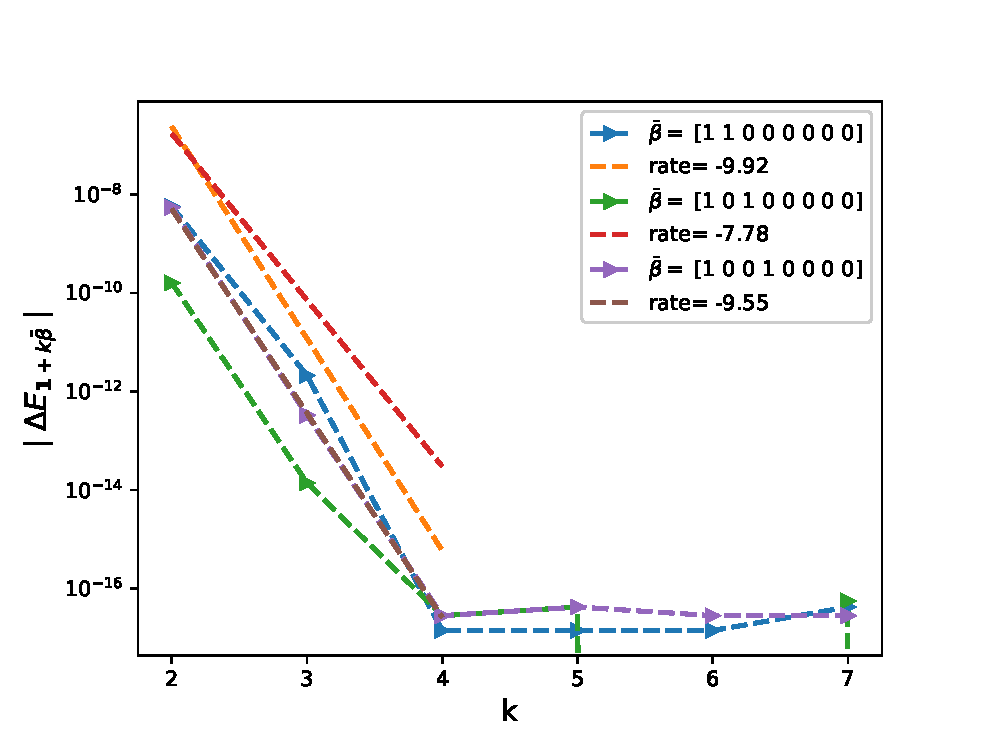
\includegraphics[width=1\linewidth]{./figures/rBergomi_mixed_error_rates/without_change_measure/N_4/H_002/mixed_difference_order2_rbergomi_4steps_H_002_K_1_totally_hierarch_with_rate_W1}
		\caption{}
		\label{fig:sub3}
	\end{subfigure}%
	\begin{subfigure}{.4\textwidth}
		\centering
		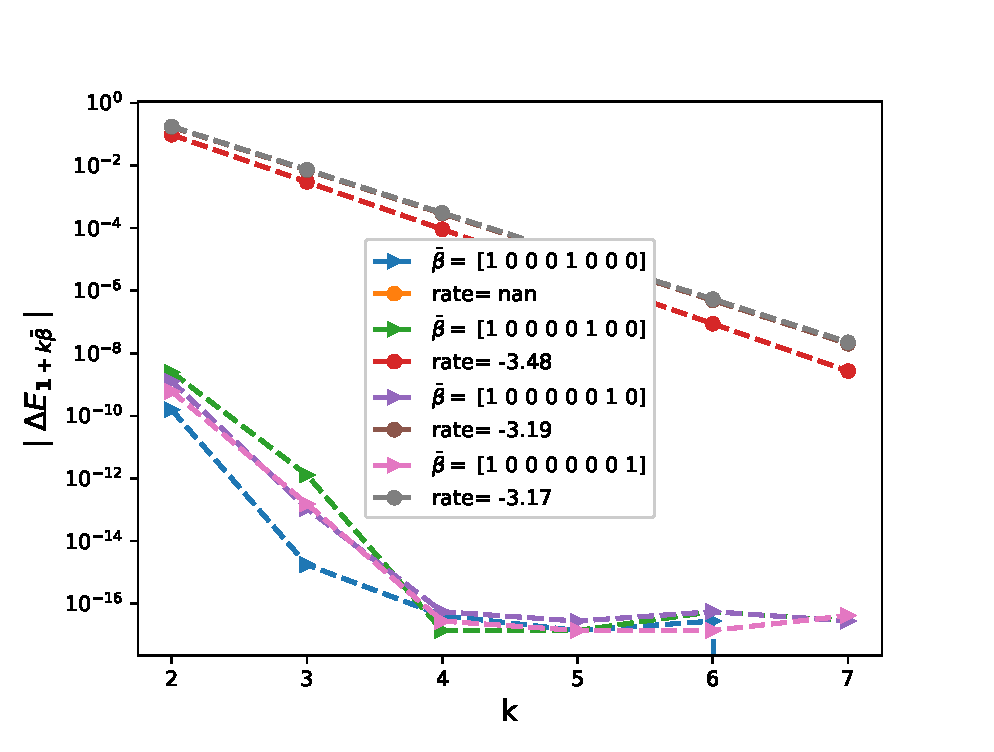
\includegraphics[width=1\linewidth]{./figures/rBergomi_mixed_error_rates/without_change_measure/N_4/H_002/mixed_difference_order2_rbergomi_4steps_H_002_K_1_totally_hierarch_with_rate_W2}
		\caption{}
		\label{fig:sub4}
	\end{subfigure}
	
	\caption{The rate of convergence of  second order differences $\abs{\Delta \text{E}_{\beta}}$ ($\beta=\mathbf{1}+k \bar{\beta}$) with respect to $W^{(1)}$ (a)  and  with respect to $W^{(2)}$ (b), for parameter set $2$ in table \ref{table:Reference solution, using MC with $500$ time steps, of Call option price under rBergomi model, for different parameter constellation.}. The number of quadrature points used in the $i$-th dimension is $N_i=2^{\beta_i-1}+1$.}
	\label{fig:second_diff_comp_K_1_H_002}
\end{figure}

\FloatBarrier

%
%\begin{remark}
%	In this paper, we limited ourselves to designing a novel alternative method  based on hierarchical adaptive sparse grids quadrature for computing option prices under the rBergomi model. Giving the significant performance gains of our novel designed algorithm, we expect that designing a method based on QMC can bring similar or more gains as  our approach.
%\end{remark}



\subsection{Brownian bridge construction}\label{sec:Brwonian bridge construction}
In the literature of adaptive sparse grids and  QMC, several hierarchical path generation methods (PGMs) or transformation methods have been proposed to reduce the effective dimension. Among these transformations, we cite  the Brownian
bridge (Bb)  construction \cite{morokoff1994quasi,moskowitz1996smoothness,caflisch1997valuation}, the principal component analysis (PCA)  \cite{acworth1998comparison} and the linear transformation (LT) \cite{imai2004minimizing}.

In our context, the Brownian motion can be constructed either sequentially using a standard random walk construction or hierarchically using   other hierarchical PGM as listed above. For our purposes, to make an effective use of MISC, which profits from anisotropy, we use the Bb construction since it produces  dimensions with different importance for MISC, contrary to random walk procedure for which all the dimension of the stochastic space have equal importance.  This transformation  reduces the effective dimension  of the problem and as a consequence accelerates the MISC procedure by reducing the computational cost.


Let us denote $\{t_i\}_{i=0}^{N}$ the grid of time steps, then the Bb construction \cite{glasserman2004monte} consists of the following: given a past value $B_{t_i}$ and a future value $B_{t_k}$, the value $B_{t_j}$ (with $t_i < t_j < t_k$) can be generated according to the formula:
\begin{equation}
B_{t_j}=(1-\rho) B_{t_i}+\rho B_{t_k}+ \sqrt{\rho (1-\rho)(k-i) \Delta t} z, \: z \sim \mathcal{N}(0,1) \COMMA
\end{equation}
where $\rho=\frac{j-i}{k-i}$.  In particular, if $N$ is a power of $2$, then given $B_0=0$, Bb generates the Brownian motion at times $T, T/2,T/4,3T/4,\dots$ according
\begin{align}\label{eq:BB construction}
	B_T&=\sqrt{T}z_1\nonumber\\
	B_{T/2}&= \frac{1}{2}(B_{0}+B_{T})+\sqrt{T/4}z_2= \frac{\sqrt{T}}{2} z_1+\frac{\sqrt{T}}{2} z_2\nonumber\\
	B_{T/4}&=\frac{1}{2} (B_{0}+B_{T/2})+\sqrt{T/8}z_3= \frac{\sqrt{T}}{4} z_1+\frac{\sqrt{T}}{4} z_2+\sqrt{T/8}z_3\nonumber\\
	\vdots \nonumber\\
\end{align}
where $\{z_j\}_{j=1}^{N}$ are independent standard normal variables.  In Bb construction scheme given by \eqref{eq:BB construction}, the most important values that determine the large scale structure of Brownian motion are the first components of $\mathbf{z} = (z_1,\dots,z_N)$.



%\begin{remark}
%In this paper, we chose to couple Brownian bridge construction with the MISC solver to reduce the effective dimension, since it is the less costly option in terms of computational work and the easiest to implement. We did not investigate the performance of MISC when coupling it with other hierarchical path generations method such as PCA or LT, which could be left as a future work that looks for the optimal PGM to couple with MISC in this context.
%\end{remark}
%


\subsection{Richardson extrapolation}\label{sec:Richardson extrapolation}


Another transformation that we coupled with MISC is Richardson extrapolation \cite{talay1990expansion}. In fact, applying level $K_\text{R}$ of Richardson extrapolation reduces dramatically the bias and as a consequence reduces the needed number of time steps $N$ used in the coarsest level to achieve a certain error tolerance. This means basically that Richardson extrapolation reduces directly the total dimension of the integration problem for achieving some error tolerance.


We  recall that the Euler scheme has weak order one so that

\begin{align}\label{Euler_weak_error}
	\abs{\expt{f(\hat{X}_T^h)}-\expt{f(X_T)} }  \leq C h
\end{align}

for some constant $C$, all sufficiently small $h$ and suitably smooth $f$. It can be easily  shown that  \eqref{Euler_weak_error} can be improved to


\begin{align}\label{Euler_weak_error_strenghten}
	\expt{f(\hat{X}_T^h)}= \expt{f(X_T)} + c h +\Ordo{h^2} \COMMA
\end{align}


where $c$ depends on $f$. 

Applying \eqref{Euler_weak_error_strenghten} with discretization step $2h$, we  obtain

\begin{align}\label{Euler_weak_error_strenghten_2h}
	\expt{f(\hat{X}_T^{2h})}= \expt{f(X_T)} + 2 c h +\Ordo{h^2} \COMMA
\end{align}

implying

\begin{align}\label{Richardson_extrapol}
	2 \expt{f(\hat{X}_T^{2h})}- \expt{f(\hat{X}_T^{h})} =\expt{f(X_T)} + \Ordo{h^2} \COMMA
\end{align}

For higher levels extrapolations, we use the following: Let us denote by $h_J=h_0 2^{-J}$ the grid sizes (where $h_0$ is the coarsest grid size), by $K_\text{R}$ the level of the Richardson extrapolation, and by $I(J,K_\text{R})$ the approximation of $\expt{f((X_T)}$ by terms up to level $K_\text{R}$ (leading to a weak error of order $K_\text{R}$), then we have the following recursion 

\begin{align}
I(J,K_\text{R})=\frac{2^{K_\text{R}}\left[I(J,K_\text{R}-1)-I(J-1,K_\text{R}-1)\right]}{2^{K_\text{R}}-1},\quad J=1,2,\dots, K_\text{R}=1,2,\dots
\end{align}



%\begin{remark}
%	We note that we did not apply Richardson extrapolation for all our numerical experiments. In fact, as it will be illustrated later in Section \ref{sec:Numerical tests}, for some parameter constellations, we can get a satisfactory small error tolerance even without applying a level $1$ of Richardson extrapolation. Those cases basically are characterized by a sufficiently small bias in the pre-asymptotic regime.	
%\end{remark}



